\documentclass[tikz,border=8pt]{standalone}
% Shared look for every TikZ diagram. Load with \input{../../tools/tikz-style.tex}
\usepackage[T1]{fontenc}
\usepackage{lmodern}
\renewcommand{\sfdefault}{lmr}  % diagrams use the same serif as the text
\usetikzlibrary{arrows.meta, positioning, shapes.geometric, calc, fit, backgrounds}
\definecolor{cblue}{HTML}{4C78A8}
\definecolor{corange}{HTML}{F58518}
\definecolor{cgreen}{HTML}{54A24B}
\definecolor{cred}{HTML}{E45756}
\definecolor{cpurple}{HTML}{B279A2}
\definecolor{cgrey}{HTML}{6B6B6B}
\tikzset{
  every picture/.style={font=\sffamily, line width=1.2pt},
  box/.style={draw=#1, fill=#1!12, rounded corners=4pt, align=center, inner sep=7pt, minimum height=1.1cm},
  box/.default=cgrey,
  arrow/.style={-{Stealth[length=3mm]}, draw=cgrey, line width=1.4pt},
  title/.style={font=\sffamily\bfseries\Large},
  note/.style={font=\sffamily\small, text=cgrey, align=center},
}
\AtBeginDocument{\hyphenpenalty=10000 \exhyphenpenalty=10000}

\begin{document}
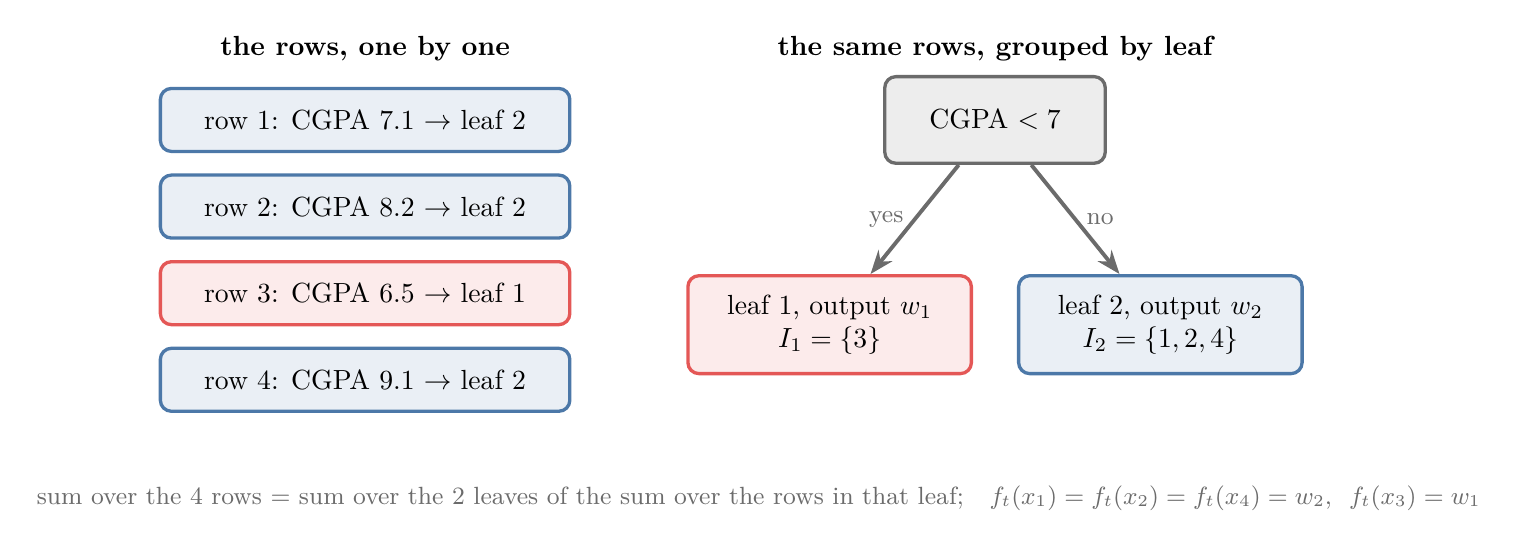
\begin{tikzpicture}[rb/.style={box=cblue, minimum width=5.2cm, minimum height=0.8cm, inner sep=4pt},
  rr/.style={box=cred, minimum width=5.2cm, minimum height=0.8cm, inner sep=4pt},
  n/.style={box=cgrey, minimum width=2.8cm}, l1/.style={box=cred, minimum width=3.6cm}, l2/.style={box=cblue, minimum width=3.6cm}]
  \node[font=\sffamily\bfseries] at (-5,0.9) {the rows, one by one};
  \node[rb] at (-5,0) {row 1: CGPA 7.1 $\rightarrow$ leaf 2};
  \node[rb] at (-5,-1.1) {row 2: CGPA 8.2 $\rightarrow$ leaf 2};
  \node[rr] at (-5,-2.2) {row 3: CGPA 6.5 $\rightarrow$ leaf 1};
  \node[rb] at (-5,-3.3) {row 4: CGPA 9.1 $\rightarrow$ leaf 2};
  \node[font=\sffamily\bfseries] at (3,0.9) {the same rows, grouped by leaf};
  \node[n] (root) at (3,0) {CGPA $< 7$};
  \node[l1] (l1) at (0.9,-2.6) {leaf 1, output $w_1$\\$I_1 = \{3\}$};
  \node[l2] (l2) at (5.1,-2.6) {leaf 2, output $w_2$\\$I_2 = \{1, 2, 4\}$};
  \draw[arrow] (root) -- node[note, left] {yes} (l1); \draw[arrow] (root) -- node[note, right] {no} (l2);
  \node[note] at (0,-4.8) {sum over the 4 rows $=$ sum over the 2 leaves of the sum over the rows in that leaf;\quad
    $f_t(x_1) = f_t(x_2) = f_t(x_4) = w_2$, \ $f_t(x_3) = w_1$};
\end{tikzpicture}
\end{document}
